\section{Problem 3}

This problem takes into account the transmission line in figure \ref{p3:TL}. The circuit illustrates a power amplifier (non-ideal voltage source with impedance $Z_S$) that feeds an antenna (load) with impedance $Z_L = 50 \Omega$ through a transmission line with characteristic impedance $Z_0=50 \Omega$, length $l=21.875 cm$ and relative permittivity of $\epsilon_r=4$ (the relative permeability is considered to be unitary $\mu_r = 1$). Additional information was achieved from measurements with a capacitive probe, they are:


\begin{itemize}
    \item As getting far from the load the voltage drops and reach a minimum at $4.75 mm$ of distance from the antenna;
    \item Beyond this point the voltage rises and reach its maximum at $36 mm$ of distance from the antenna with $\text{VSWR}=3$.
\end{itemize}

\begin{figure}[H] 
\centering
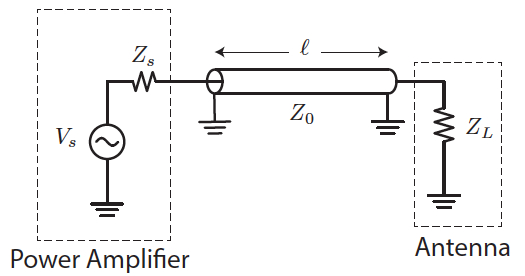
\includegraphics[width=9cm]{images/tl_ckt_p3.png}
\caption{Transmission line for problem 3.}
\label{p3:TL} 
\end{figure}

\subsection{Power amplifier operating frequency}

It known that the distance between the maximum voltage and its minimum is equivalent to a quarter of wavelength, so: $\Delta z = z_{max} - z_{min} = \frac{\lambda}{4} = 31.25mm$ and finally $\lambda = 125mm$. Therefore the operating frequency is given by equation \ref{p3:opfreq}: 

\begin{equation} \label{p3:opfreq}
    f = \frac{v}{\lambda} = \frac{c}{\lambda} \frac{1}{\sqrt{\epsilon_r \mu_r}} = \frac{3 \times 10^8}{125 \times 10^{-3}} \frac{1}{\sqrt{4 \times 1}} = 1.2 GHz
\end{equation}

\subsection{Antenna impedance at operating frequency}

The impedance in any given point of the line is given by the equation \ref{p3:imp}.

\begin{equation} \label{p3:imp}
    Z(z) = Z_0 \frac{1+\rho_L e^{2j \beta z}}{1 -\rho_L e^{2j \beta z}}
\end{equation}

Considering that the antenna is located at $z=0$, the exponential term turn to be $e^{2j \beta z}=1$ and the equation \ref{p3:imp} becomes \ref{p3:antenna}.

\begin{equation} \label{p3:antenna}
    Z_L = Z_0 \frac{1+\rho_L}{1 -\rho_L}
\end{equation}

Although the reflection coefficient $\rho_L$ remains unknown and it has a module and phase ($\rho_L = |\rho_L| e^{j\theta}$). Its module can be computed by the equation \ref{p3:vswrrho} while the phase can be found by the equation \ref{p3:zminrho} that relate it with the distance whose occurs a voltage minimum.

\begin{equation} \label{p3:vswrrho}
    \text{VSWR} = \frac{1+|\rho_L|}{1-|\rho_L|} \Rightarrow |\rho_L| = \frac{\text{VSWR}-1}{\text{VSWR}+1}
\end{equation}

\begin{equation} \label{p3:zminrho}
    z_{max} = \frac{\theta \lambda}{4\pi} \Rightarrow \theta = \frac{4 \pi z_{max}}{\lambda}
\end{equation}

For $\text{VSWR}=3$, implies $|\rho_L|=0.5$ and bearing in mind the results from the previous section, we have the phase $\theta = 3.6191 rad$. Therefore $\rho_L = 0.5 e^{j3.6191}$ and regarding the equation \ref{p3:antenna}, finally $Z_L = 20.569 e^{-j0.5497} \Omega = 17.538 - j10.74 \Omega$.

Plotting the voltage waveform (figure \ref{ads:plot:vswr}) in both end of the line we observed that indeed the VSWR is 3.

\begin{figure}[H] 
\centering
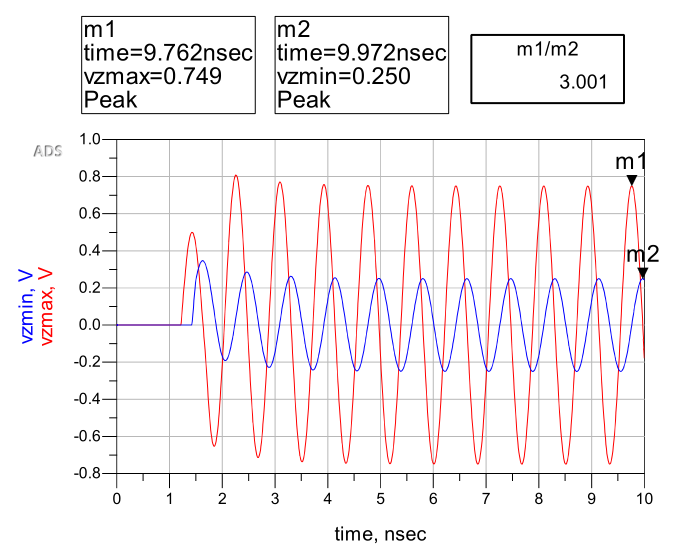
\includegraphics[width=9cm]{images/lab1_p3_vswr.png}
\caption{Voltage at source and load with sinusoidal excitation.}
\label{ads:plot:vswr} 
\end{figure}

\subsection{Mathematical expression of voltage along the line}

Considering a lossless line ($\alpha = 0$), the voltage along the line takes the form:

\begin{center}
    $V(-z) = V^+ e^{-\gamma z} +V^- e^{+ \gamma z}$ \\ \vspace{1pt}
    $V(-z) = V^+ e^{-j\beta z} +V^- e^{+ j\beta z}$ \\ \vspace{1pt}
\end{center}
\begin{equation} \label{p3:expvolt1} 
     V(-z) = V^+ e^{+ j\beta z} (1 + \rho_L e^{-2j \beta z})
\end{equation}

At the source ($z=l$) the previous expression becomes as follow (also the voltage provided by the source is the one after the voltage drop at the source impedance):

\begin{equation} \label{p3:expvolt2}
    V(-l) = V^+ e^{+ j\beta l} (1 + \rho_L e^{-2j \beta l})  = V_S - Z_S I_S
\end{equation}

While the source current is the composition of the incident and reflected current:

\begin{center} 
    $I_S = I^+(-l) + I^-(-l) = \frac{V^+(-l) + V^-(-l)}{Z_0}$
\end{center}

The expression \ref{p3:expvolt2} becomes:

\begin{center} 
    $V(-l) = \frac{V^+ e^{+j\beta l}}{Z_0} (1- \rho_L e^{+2j \beta l})$
\end{center}

Then:

\begin{equation} \label{p3:expvolt5}
    V^+ = V_S e^{-j \beta l} [(1+\rho_L e^{-2j\beta l})+\frac{Z_S}{Z_0}(1-\rho_L e^{-2j\beta l})]^{-1}
\end{equation}

Once $V^+$ is a known value, the expression \ref{p3:expvolt1} will allow us to trace the voltage envelope with a variable $z$ that will limit the voltage at any point and any time of the line.

The mathematical expression for the voltage along the line was derived in the Display Window environment of ADS, resulting in the figure \ref{calculus}. Once the variables were stored in the ADS work space, the waveform from figure \ref{p3:waveform} could be plotted, resulting in the combination of the upper and lower voltage envelope due to the stationary wave and the voltage waveform across the line in a given time (selected in a slider) bounded inside the envelope. Even varying the time instant of analysis, the voltage still bounded inside the envelope across all line.

\begin{figure}[H] 
\centering
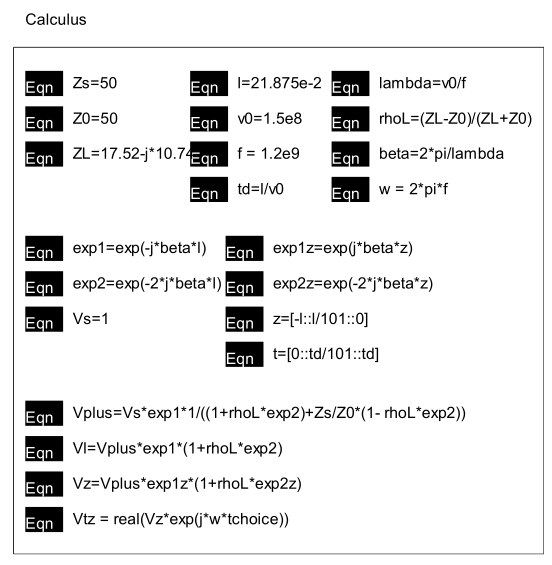
\includegraphics[width=9cm]{images/calculus.png}
\caption{Set of equations in the Display Window environment of ADS.}
\label{calculus} 
\end{figure}

\begin{figure}[H] 
\centering
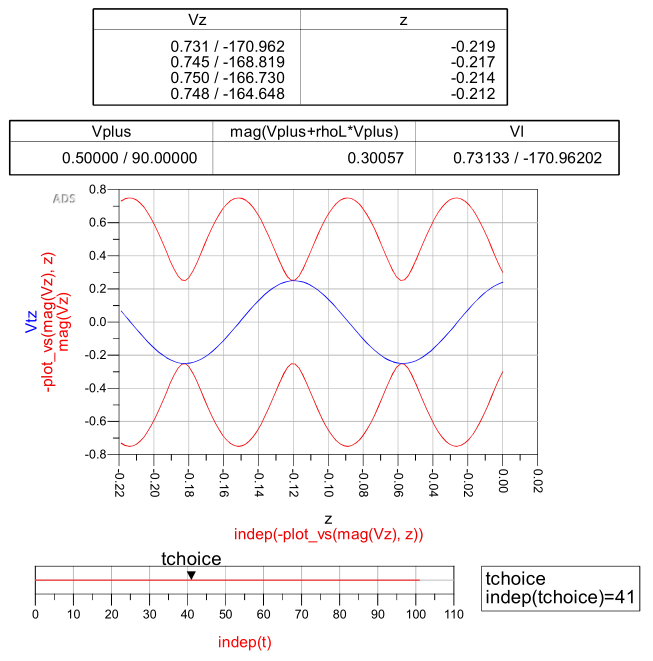
\includegraphics[width=12cm]{images/lab1_p3_waveform.png}
\caption{Waveform for the voltage along the line.}
\label{p3:waveform} 
\end{figure}